\documentclass[a4paper,twoside,11pt]{article}
\usepackage{a4wide,graphicx,fancyhdr,amsmath,amssymb,placeins}
\usepackage{listings}
\usepackage{color}
\usepackage{enumitem}
\usepackage{amsmath}
\usepackage{textcomp}
\usepackage{caption,subcaption}

%----------------------- Macros and Definitions --------------------------

\setlength\headheight{20pt}
\addtolength\topmargin{-10pt}
\addtolength\footskip{20pt}

\newcommand{\N}{\mathbb{N}}
\newcommand{\ch}{\mathcal{CH}}
\newcommand{\cpp}{{\tt C++} }

\newcommand{\solution}[1][todo]{\noindent{\bf Solution to Exercise #1:}}
\newcommand{\todo}[1]{\textcolor{red}{#1}}

\renewcommand{\lstlistingname}{Codeblock}
\captionsetup[lstlisting]{font={small,tt}}

\fancypagestyle{plain}{%
\fancyhf{}
\fancyhead[LO,RE]{\sffamily\bfseries\large technische universiteit eindhoven}
\fancyhead[RO,LE]{\sffamily\bfseries\large 2IW02 RTSD}
\fancyfoot[LO,RE]{\sffamily\bfseries\large department of mathematics and computer science}
\fancyfoot[RO,LE]{\sffamily\bfseries\thepage}
\renewcommand{\headrulewidth}{0pt}
\renewcommand{\footrulewidth}{0pt}
}

\pagestyle{fancy}
\fancyhf{}
\fancyhead[RO,LE]{\sffamily\bfseries\large technische universiteit eindhoven}
\fancyhead[LO,RE]{\sffamily\bfseries\large 2IW02 RTSD}
\fancyfoot[LO,RE]{\sffamily\bfseries\large department of mathematics and computer science}
\fancyfoot[RO,LE]{\sffamily\bfseries\thepage}
\renewcommand{\headrulewidth}{1pt}
\renewcommand{\footrulewidth}{0pt}

%-------------------------------- Title ----------------------------------

\title{\vspace{-\baselineskip}\sffamily\bfseries Exercise 2}
\author{
	Rick Veens \qquad Studentno: 0912292\\
	\texttt{r.veens@student.tue.nl}
	\and
	Huib Donkers \qquad Studentno: 0769015\\
	\texttt{h.t.donkers@student.tue.nl}
}

\date{\today}

\definecolor{listinggray}{gray}{0.9}
\definecolor{lbcolor}{rgb}{0.9,0.9,0.9}
\lstset{
backgroundcolor=\color{lbcolor},
    tabsize=4,    
%   rulecolor=,
    language=[GNU]C++,
        basicstyle=\scriptsize,
        upquote=true,
        aboveskip={1.5\baselineskip},
        columns=fixed,
        showstringspaces=false,
        extendedchars=false,
        breaklines=true,
        prebreak = \raisebox{0ex}[0ex][0ex]{\ensuremath{\hookleftarrow}},
        frame=single,
        numbers=left,
        showtabs=false,
        showspaces=false,
        showstringspaces=false,
        identifierstyle=\ttfamily,
        keywordstyle=\color[rgb]{0,0,1},
        commentstyle=\color[rgb]{0.026,0.112,0.095},
        stringstyle=\color[rgb]{0.627,0.126,0.941},
        numberstyle=\color[rgb]{0.205, 0.142, 0.73},
%        \lstdefinestyle{C++}{language=C++,style=numbers}’.
}

% geen stomme indents bij \par
\setlength{\parindent}{0cm}

%--------------------------------- Text ----------------------------------

\begin{document}
\maketitle

\section{Timers}
\subsection{Model}
\todo{Plaatjes/uitleg over gebruikte model/code?}

\subsection{Questions}
\begin{enumerate}
 \item Measured over \todo{$n$} intervals, the variation is \todo{$\sigma$}. See figure~\ref{fig:interval-jitter} for the exact distribution.
 
 \item This jitter is the result of simulating a real time OS in an environment that is not real time. Realtime requirements are not met. \todo{Meer uitleg?} Additionally, the way we measure the intervals can also introduce more jitter in the results than there actually is. \todo{Meer uitleg}
 
 \item \todo{depends on the variation, it's probably too big}
 
 \item No. Our host system has different priorities, it does not guarantee to meet real time requirements. \todo{Meer uitleg? Is ``No'' wel het goeie antwoord eigenlijk?}
 
 
\end{enumerate}

\begin{figure}
 \centering
 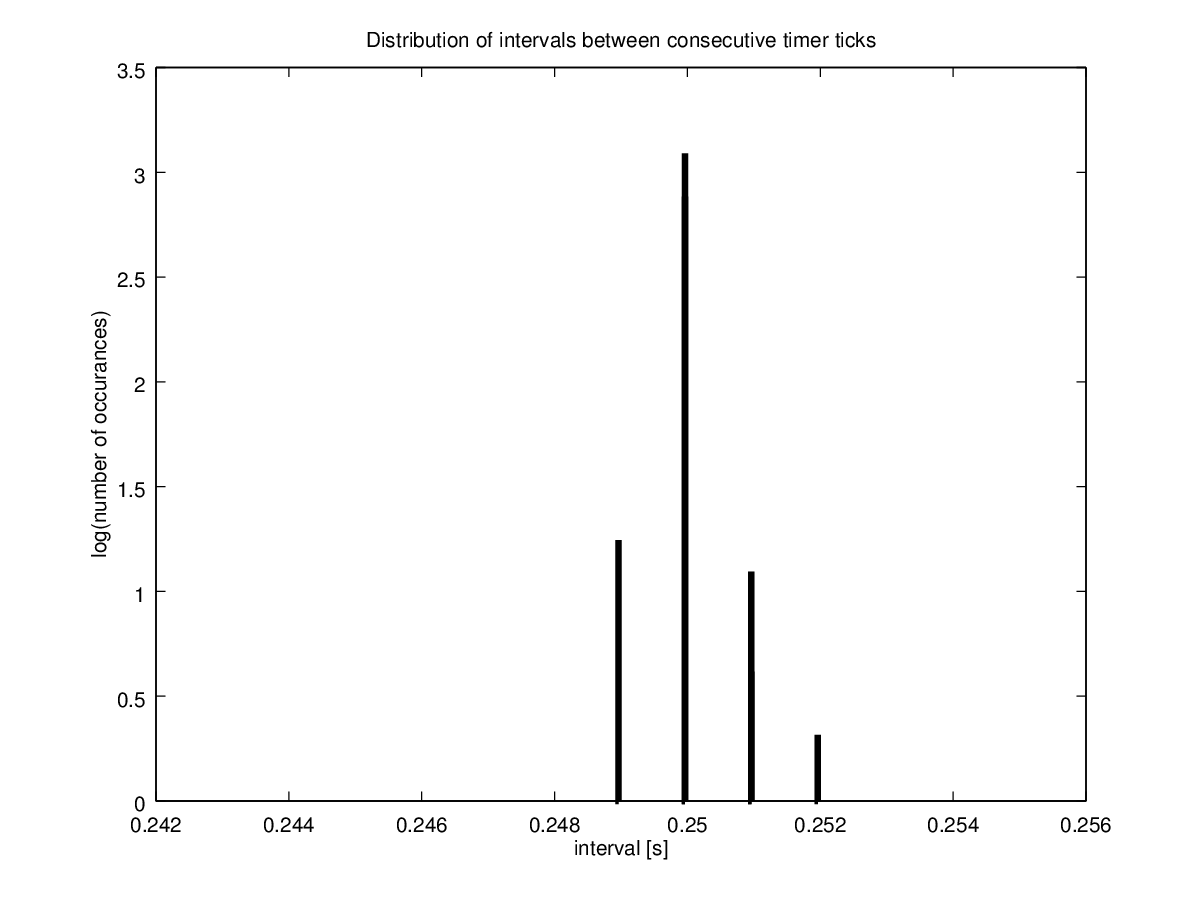
\includegraphics{./img/interval-jitter.png}
 \caption{Distribution of intervals.}
 \label{fig:interval-jitter}
\end{figure}

\subsection{Validation}
\todo{Uitleg}

\subsection{Questions}
\begin{enumerate}
 \item \todo{todo}
 \item \todo{todo}
 \item \todo{todo}
\end{enumerate}

\section{JIWYIO Linkdrivers}
\subsection{JIWYIO driver components}
\todo{Uitleg}

\subsection{Questions}
\begin{enumerate}
 \item \todo{todo}
 \item \todo{What!? ... You want us to tell you how the tool should work? This isn't software specification, and even worse, the tool is not the subject, it's the tool...}
 \item \todo{Zucht...}
\end{enumerate}

\subsection{JIWYIO driver componenets in the lab}
\todo{report}

\subsection{Questions}
\begin{enumerate}
 \item \todo{todo}
 \item \todo{todo}
\end{enumerate}

\section{Controlling JIWY with QNX \& CSP}
\subsection{Test at the lab}
\todo{report}

\subsection{Questions}
\begin{enumerate}
 \item \todo{todo}
 \item \todo{todo}
\end{enumerate}

\subsection{Further functionality}
\todo{explain we didn't have time and it's not our fault}

\subsection{Questions}
\begin{enumerate}
 \item \todo{todo}
 \item \todo{todo}
 \item \todo{todo}
 \item \todo{todo}
\end{enumerate}

\end{document}
